%!TEX root = ../../main.tex

\chapter{Theoretische Grundlagen}

\section{Unwucht}
Eine Unwucht ist eine Rotation, welche bei einem rotierenden Körper nicht in der Hauptträgheitsachse stattfindet, sondern leicht versetzt.
Unwuchten erzeugen drehzahlabhängigen Vibrationen, welche zu einem erhöhten Verschleiß, bis hin zu der Zerstörung des gesamten Systems führen können.
Diese enstehen bei einem Rotationskörper, wenn sich der Schwerpunkt nicht auf der Rotationsachse befindet und damit die Fliehkräfte nicht mehr gegenseitig aufgehoben werden können. \cite{unwucht_wiki:2011}

Es wird zwischen zwei Arten von Unwuchten unterschieden:
\begin{itemize}
    \item Statische Unwucht
    \item Dynamische Unwucht
\end{itemize}

Statische Unwucht entsteht, wenn an einem vollkommen ausgewuchteten Rotationskörper auf der Radialebene eine Schwerpunktverlagerung stattfindet. Beispielhaft ist dies in Abbildung \ref{fig:static_imbalance} dargestellt.
Dadurch entstehen kreisförmige Schwingungen rechtwinklig zur Rotationsachse.
\begin{figure}[H]
    \centering
    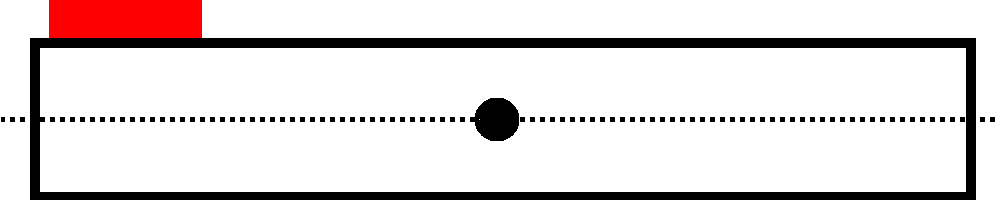
\includegraphics[width=8cm]{images/chapter/02/static_imbalance.png}
    \caption{Bildliche Darstellung einer statischen Unwucht}
    \label{fig:static_imbalance}
\end{figure}

Die dynamische Unwucht tritt auf, wenn sich zwei gleich große, aber zueinander entgegengesetzt liegende Unwuchten in unterschiedlichen Radialebenen befinden, wie in Abbildung \ref{fig:dynamic_imbalance} abgebildet.
Hierdurch fängt die Rotationsachse an sich hin- und herzubewegen, während der Schwerpunkt des Rotationskörpers in Ruhelage verbleibt.
Diese Art der Unwucht macht sich jedoch erst bei sehr hohen Drehzahlen bemerkbar \cite[S. 8]{vibromatrix:2007}.
\begin{figure}[H]
    \centering
    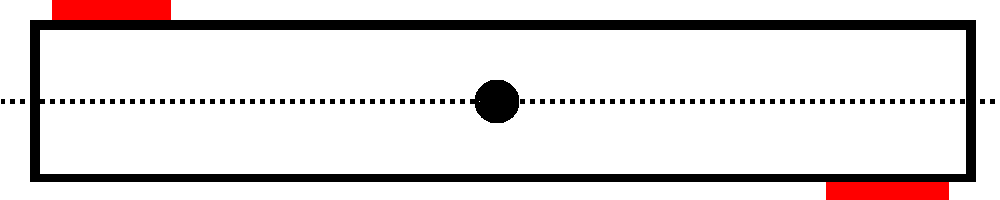
\includegraphics[width=8cm]{images/chapter/02/dynamic_imbalance.png}
    \caption{Bildliche Darstellung einer dynamischen Unwucht}
    \label{fig:dynamic_imbalance}
\end{figure}

\section{Mikrocontrollerplattform Arduino}
